%**************************************************************************
% WSC 2026 Poster Extended Abstract -- SEGUNDO abstract (simulacao GNSS-denied)
% Numeros: gnss_wsc250_summary.json + gnss_wsc250_fg_summary.json
%**************************************************************************
\documentclass{wscposterproc}

\usepackage{graphicx}
\usepackage{booktabs}
\usepackage{caption}
\captionsetup{font=scriptsize,skip=2pt,labelfont=bf}
\usepackage{mathptmx}
\usepackage[T1]{fontenc}
\usepackage[pdftex,colorlinks=true,urlcolor=blue,citecolor=black,anchorcolor=black,linkcolor=black]{hyperref}

\begin{document}

\WSCpagesetup{Machado and Kuroswiski}

\title{A MULTI-SENSOR LOCKSTEP SIMULATION ENVIRONMENT FOR DEVELOPING\\
GNSS-DENIED UAS NAVIGATION}

\author{
Pedro Henrique Blatt Machado\\[2pt]
Instituto Tecnol\'ogico de Aeron\'autica (ITA), S\~ao Jos\'e dos Campos, SP, BRAZIL\\
\email{pedro.blatt@ita.br}
\and
Andr\'e Kuroswiski\\[2pt]
Instituto de Controle do Espa\c{c}o A\'ereo (ICEA), S\~ao Jos\'e dos Campos, SP, BRAZIL\\
\email{andre.kuroswiski@icea.gov.br}
}

\maketitle

\section*{ABSTRACT}
Developing navigation for GNSS-denied urban flight needs an environment that can
withhold GNSS on demand, expose every remaining sensor, and still provide exact
ground truth.
We present such an environment: a high-fidelity urban scene in Cosys-AirSim coupled
in lockstep to an unmodified PX4 autopilot, where GNSS aiding is revoked
\emph{during flight} through a single estimator parameter while inertial,
barometric, magnetic, ranging, and visual streams are logged against simulator
truth at $20$\,Hz.
Because the autopilot is the real flight stack and the coupling is MAVLink
throughout, the same scenario definition drives software- and hardware-in-the-loop
without modification.
We demonstrate the environment with an inertial drift baseline
($|e| \approx 0.15\,t^{1.92}$ over $3$ runs) and by replaying a factor-graph
smoother on the identical denied windows, reducing median terminal error from
$88$\,m to $3.1$\,m.
The environment, not any single estimator, is the contribution; absolute values
are simulator-specific.

\section{INTRODUCTION}
\label{sec:intro}
Estimators that fuse inertial, visual, and ranging measurements in a factor-graph
formulation~\cite{dellaert2017factor} are a leading route to urban flight where
GNSS is unreliable.
Developing them is limited less by estimator theory than by obtaining synchronized
multi-modal measurements during a controlled GNSS outage, with position truth
accurate enough to grade the result.
Flight tests supply realism but no truth and no repeatability; replayed public
datasets supply neither a controllable outage nor a closed loop through a real
autopilot.

This abstract contributes a simulation environment that closes that gap.
Its properties are: (i)~lockstep coupling between a photorealistic urban scene and
an unmodified PX4 flight stack; (ii)~GNSS revocation as a scenario variable applied
in flight, leaving the sensor model untouched; (iii)~synchronized logging of the
remaining sensor suite against ground truth, in the form a factor-graph smoother
consumes; and (iv)~a MAVLink-only interface, so scenarios migrate to
hardware-in-the-loop unchanged.

\section{SIMULATION ENVIRONMENT}
\label{sec:method}

\vspace{-2mm}
\begin{figure}[htb]
\centering
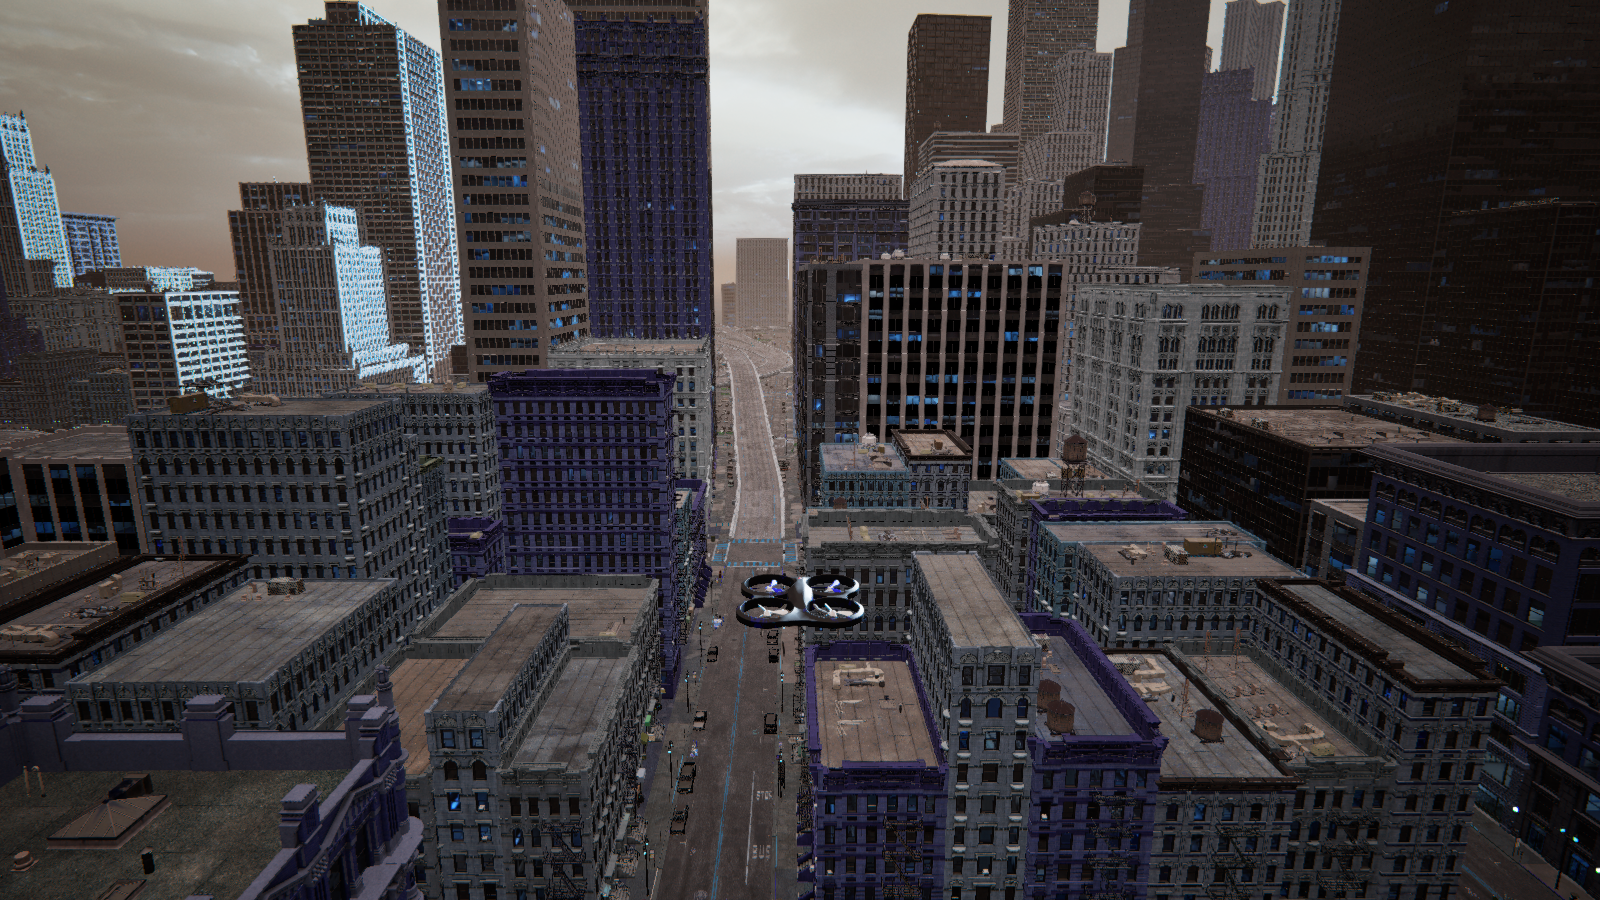
\includegraphics[width=0.52\textwidth]{../figures/wsc26_gnss_scene.png}
\vspace{-2mm}
\caption{Simulated urban scene. Demonstration flights use $250$\,m AGL so drift is
not confounded by collisions with the high-rise canopy.}
\label{fig:scene}
\end{figure}
\vspace{-3mm}

Vehicle dynamics, sensors, and the urban scene (Figure~\ref{fig:scene}) come from
Cosys-AirSim~\cite{jansen2023cosys}.
State estimation and control come from PX4 SITL, coupled over TCP in lockstep so
simulator and autopilot never free-run relative to each other.
A MAVSDK client commands the profile---arm, climb to $250$\,m, then a straight
$250$\,m leg---and logs the EKF2 estimate against simulator truth.
Estimate and truth are time-aligned with a measured transport delay before errors
are formed.

\textbf{GNSS revocation as a scenario variable.}
Outages clear the estimator's GNSS fusion mask at a configured ground-truth point,
without restarting the autopilot or altering the simulated receiver, so only the
estimator is perturbed.
The height reference is moved to barometric before flight (reboot-scoped), because
leaving it at its GNSS default removes every altitude source when GNSS is cut.

\textbf{Recorded streams.}
Each run logs local position, truth, raw inertial, barometric and magnetic
measurements, and per-sweep LiDAR structure on one time base.
Repetitions reuse a warm estimator that has reconverged with GNSS aiding before each
outage; fusion is restored between flights so denied windows remain independent even
when the autopilot process is not restarted.

\section{DEMONSTRATION}
\label{sec:results}

\vspace{-2mm}
\begin{figure}[htb]
\centering
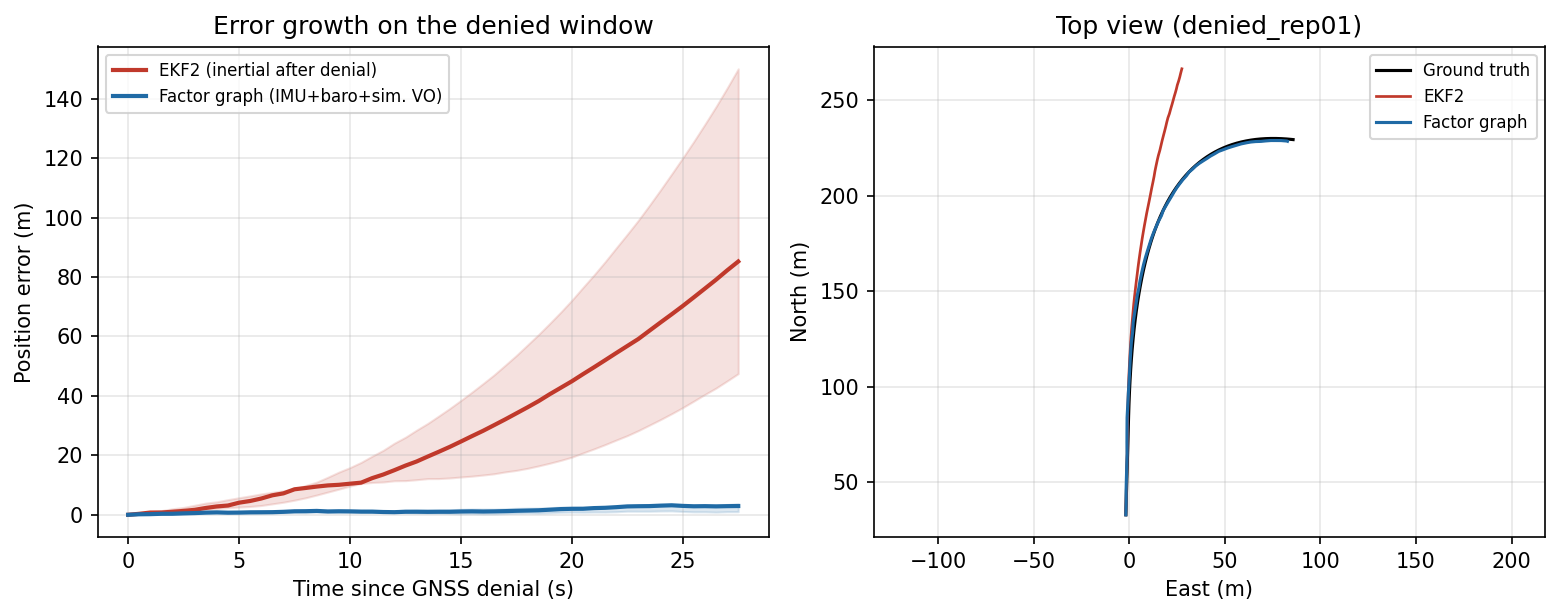
\includegraphics[width=0.92\textwidth]{../figures/gnss_wsc250_fg.png}
\vspace{-2mm}
\caption{Left: position error after GNSS denial---EKF2 inertial baseline versus a
factor-graph smoother on the same logs (median and p05--p95, $N{=}3$).
Right: top view for a representative run.}
\label{fig:fg}
\end{figure}
\vspace{-3mm}

Over $3$ repetitions, EKF2 position error during the outage grows as
$|e| \approx 0.15\,t^{1.92}$, reaching $86$\,m median ($66$--$308$) after about
$33$\,s---the inertial reference a navigation estimator must beat.
As a first consumer of the logged streams, we replay a batch factor-graph smoother
with IMU and barometric factors from the CSV plus simulated visual relative-pose
factors (ground truth with $0.12$\,m noise), standing in for a VIO front-end until
camera logs are wired.
On the same denied windows the smoother cuts median terminal error from $88$\,m to
$3.1$\,m (about $28\times$; Figure~\ref{fig:fg}), showing that the environment
supports graded comparison of estimator structure under a controlled outage.

\section{CONCLUSIONS AND ONGOING WORK}
\label{sec:concl}
The environment supplies controllable outages, synchronized sensing, exact truth, and
repeatability with a real autopilot in the loop.
Absolute drift reflects the simulator's inertial noise model rather than a specific
airframe.
Ongoing work replaces the simulated visual factors with a real image front-end on
the same scenarios, extends revocation toward receiver-level urban multipath, and
moves the profiles to hardware-in-the-loop unchanged over MAVLink.

\enlargethispage{30mm}
\vspace{-2mm}
{\fontsize{9}{10.5}\selectfont
\bibliographystyle{wsc}
\bibliography{wsc26refs}
}

\end{document}
